% !TEX root =  ../main_manuscript.tex

\section{Results}
\label{sec:results}
From the joint model fitted to the PRIAS dataset, we found that both $\log_2 \{\mbox{PSA} + 1\}$ velocity,  and log odds of having $\mbox{DRE} > \mbox{T1c}$  were significantly associated with the hazard of cancer progression. For any patient, an increase in $\log_2 \{\mbox{PSA} + 1\}$ velocity from −0.03 to 0.16 (first and third quartiles of the fitted velocities, respectively) corresponds to a 1.92 fold increase in the hazard of cancer progression. Whereas, an increase in log odds of $\mbox{DRE} > \mbox{T1c}$ from -6.65 to -4.36 (first and third quartiles of the fitted log odds, respectively) corresponds to a 1.40 fold increase in the hazard of cancer progression. Parameter estimates, and area under the receiver operating characteristic curve are presented in detail in Appendix B of the supplementary material.

\subsection{Utility of Personalized Decision Making}
From the simulation study, we obtain the number of biopsies, and the delay in detection of cancer progression for 500 x 250 test patients, due to various schedules. The corresponding, median number of biopsies and delay are shown in Figure \ref{fig:better_balance_results}. The general trend is that more biopsies are required to have a smaller delay in detection. In addition, the personalized and PRIAS approaches seem to better balance the number of biopsies, and the delay, than the fixed schedules. We next detail the results for the most widely used annual and PRIAS schedules, and compare them with personalized approach with risk thresholds of 5\% and 10\%, and threshold chosen using $\mbox{F}_1$ score. The rest are presented in Table of Apenndix????

\begin{figure}[!htb]
\captionsetup{justification=justified}
\centerline{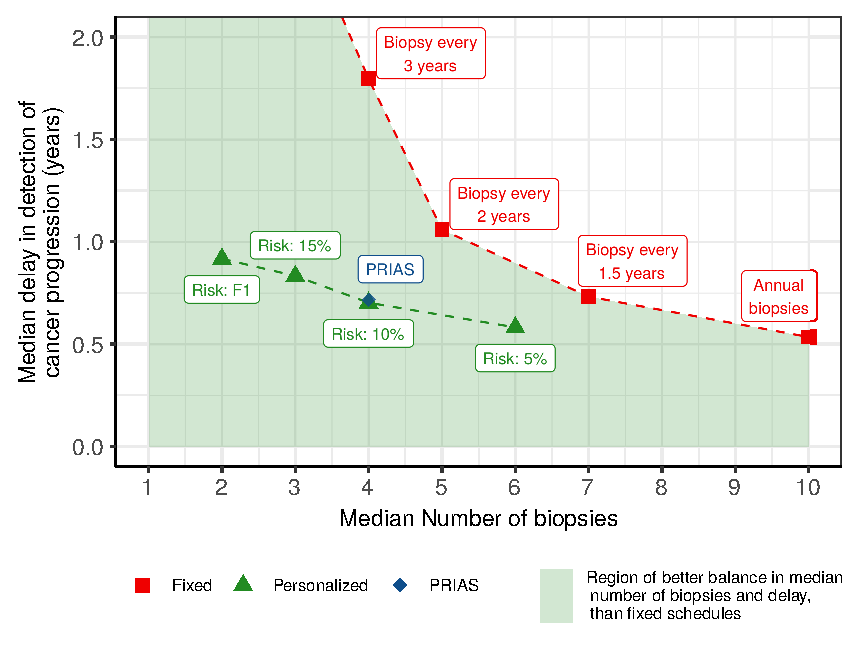
\includegraphics[width=\columnwidth]{images/better_balance_results.eps}}
\caption{Median number of biopsies scheduled by various fixed scheduling approaches (red squares) in practice, PRIAS (blue rhombus), and personalized schedules (green triangles), over a follow-up of 10 years, and the corresponding median delay in detection of cancer progression. An ideal schedule (in blue) will schedule only 1 biopsy, exactly at the true time of cancer progression. We intend to better balance the number of biopsies and the delay, than in practice currently, using personalized decision making for biopsies.}
\label{fig:better_balance_results}
\end{figure}

Since patients have varying cancer progression speeds, the utility of different schedules also varies with it. In order to highlight these differences we divide results for three types of patients, as per their time of cancer progression. They are \textit{fast, intermediate,} and \textit{slow progressing} patients. Although such a division can only be done retrospectively in a simulation setting, we do it only for the purpose of illustration. In the simulated patients, we observed that for roughly 50\% of the patients cancer progression did not take place in the 10 year follow-up (supported by kaplam meier, and figure in supplementary ???). These could be seen as patients with a slow speed of cancer progression. Roughly 30\% of the patients obtain cancer progression within first 3.5 years. These could be high risk patients who choose AS instead of immediate treatment, or patients with an initially misdiagnosed state of cancer \cite{cooperberg2011outcomes}. We consider these as fast progressing patients. We label the progression speed of the remaining 20\% patients with progression times between 3.5 and 10 years as intermediate speed. The boxplots in Figure~\ref{fig:sim_res_combined}, show the variation in the number of biopsies, and the delay in detection of cancer progression, in years (time of last biopsy - true time of cancer progression) due to various biopsy schedules, for these three types of patients.

\begin{figure}[!htb]
\captionsetup{justification=justified}
\centerline{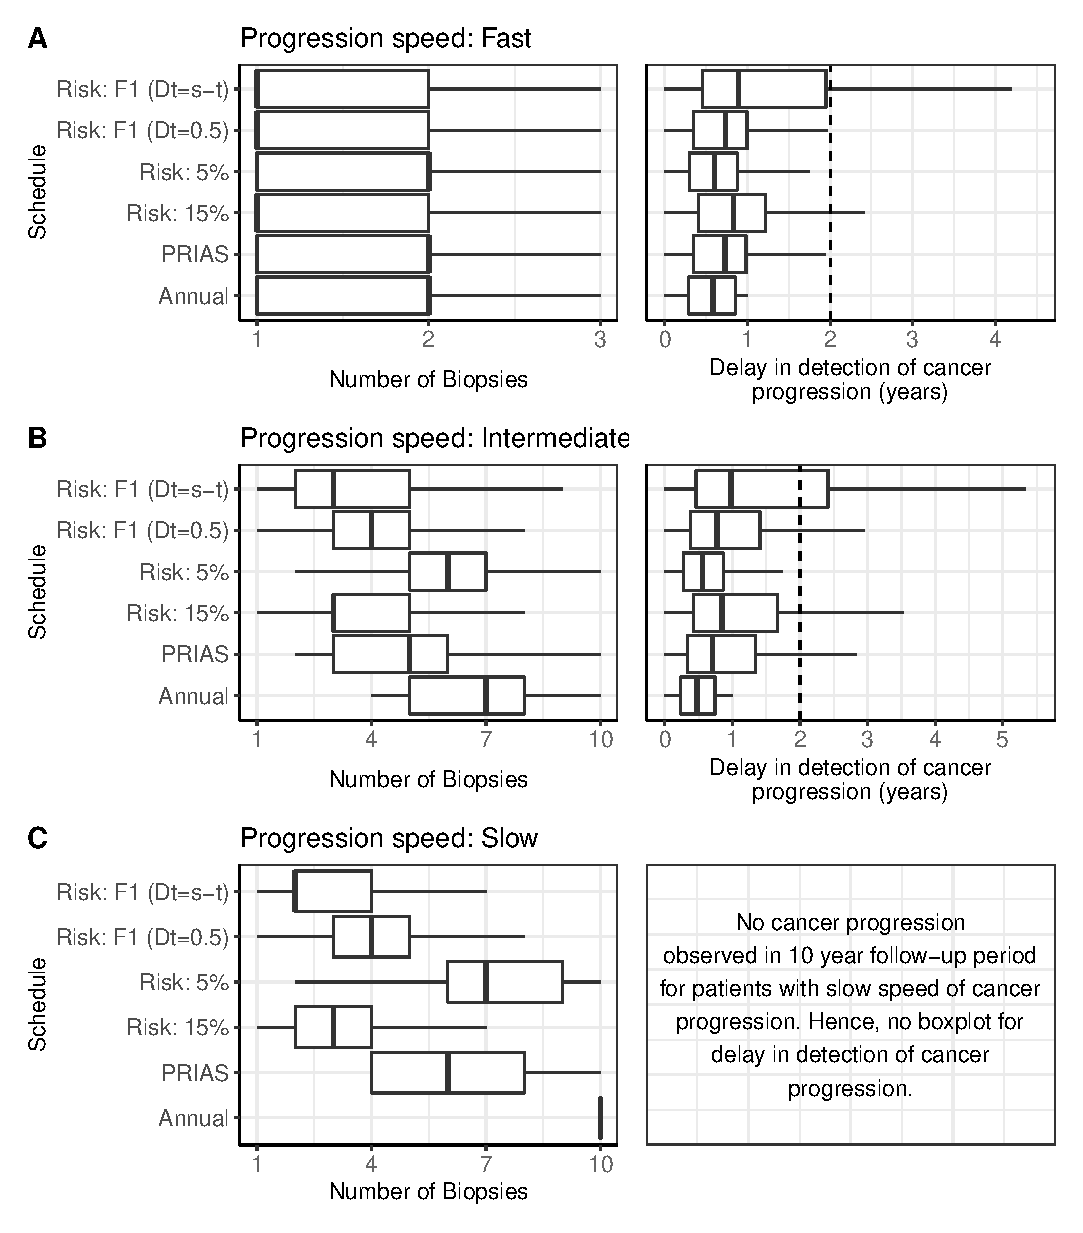
\includegraphics[width=\columnwidth]{images/sim_res_combined.eps}}
\caption{Boxplot showing variation in number of biopsies, and the delay in detection of cancer progression, in years (time of last biopsy - true time of cancer progression) for various biopsy schedules. Biopsies are conducted until cancer progression is detected. \textbf{Panel~A:} results for simulated patients who had a faster speed of cancer progression, with progression times between 0 and 3.5 years. \textbf{Panel~B:} results for simulated patients who had an intermediate speed of cancer progression, with progression times between 3.5 and 10 years. \textbf{Panel~C:} results for simulated patients who did not have cancer progression in the 10 years of follow-up. \textbf{Types of personalized schedules:} Risk:~10\% and Risk:~5\% approaches, schedule biopsy if the risk of cancer progression at a visit is more than 10\% and 5\%, respectively. Risk:~F1 works similar as previous, except that the risk threshold is chosen by maximizing $\mbox{F}_1$ score (see \hyperref[sec:methods]{Methods}). Annual corresponds to a schedule of yearly biopsies and PRIAS corresponds to biopsies as per PRIAS protocol (see \hyperref[sec:introduction]{Introduction}).}
\label{fig:sim_res_combined}
\end{figure}

For \textit{fast progressing} patients (Panel~A,~Figure~\ref{fig:sim_res_combined}), we can see that the personalized schedules have a median of one biopsy compared to two biopsies for PRIAS and annual schedule. Despite this, the delay due to personalized schedule with 10\% risk threshold is similar to that of PRIAS schedule. 

For \textit{intermediate progressing} patients (Panel~A,~Figure~\ref{fig:sim_res_combined}), we can see that personalized schedules with a small risk threshold such as 5\% risk conduct many more biopsies than other personalized schedules. Consequently, their performance with respect to the delay in detection of progression is similar to that of annual schedule. However, personalized schedule with slightly higher risk (10\%) and risk chosen using $\mbox{F}_1$ score, schedule a median of 3 and 4 biopsies each, respectively. This is despite the fact that the delay in detection of cancer progression due to the schedule with 10\% risk threshold is similar to that of the PRIAS schedule. However, the PRIAS schedule schedules an extra biopsy (median of 5 biopsies).

The patients who are at most advantage with the personalized schedules are the \textit{slow progressing} patients (50\% of the total patients). In Panel~C of Figure~\ref{fig:sim_res_combined} we can see that the annual schedule may lead to 10 unnecessary biopsies for all such patients. The PRIAS schedule, schedules a median of 6 unnecessary biopsies. In comparison the personalized schedules using 10\% risk threshold and risk chosen using $\mbox{F}_1$ score, schedule only 2 and 4 biopsies, respectively.
